
\documentclass[a4paper,11pt]{article}
\usepackage[a4paper, margin=8em]{geometry}

% usa i pacchetti per la scrittura in italiano
\usepackage[french,italian]{babel}
\usepackage[T1]{fontenc}
\usepackage[utf8]{inputenc}
\frenchspacing 

% usa i pacchetti per la formattazione matematica
\usepackage{amsmath, amssymb, amsthm, amsfonts}

% usa altri pacchetti
\usepackage{gensymb}
\usepackage{hyperref}
\usepackage{standalone}

% imposta il titolo
\title{Appunti Calcolo Numerico}
\author{Luca Seggiani}
\date{2025}

% disegni
\usepackage{pgfplots}
\pgfplotsset{width=10cm,compat=1.9}

% imposta lo stile
% usa helvetica
\usepackage[scaled]{helvet}
% usa palatino
\usepackage{palatino}
% usa un font monospazio guardabile
\usepackage{lmodern}

\renewcommand{\rmdefault}{ppl}
\renewcommand{\sfdefault}{phv}
\renewcommand{\ttdefault}{lmtt}

% disponi il titolo
\makeatletter
\renewcommand{\maketitle} {
	\begin{center} 
		\begin{minipage}[t]{.8\textwidth}
			\textsf{\huge\bfseries \@title} 
		\end{minipage}%
		\begin{minipage}[t]{.2\textwidth}
			\raggedleft \vspace{-1.65em}
			\textsf{\small \@author} \vfill
			\textsf{\small \@date}
		\end{minipage}
		\par
	\end{center}

	\thispagestyle{empty}
	\pagestyle{fancy}
}
\makeatother

% disponi teoremi
\usepackage{tcolorbox}
\newtcolorbox[auto counter, number within=section]{theorem}[2][]{%
	colback=blue!10, 
	colframe=blue!40!black, 
	sharp corners=northwest,
	fonttitle=\sffamily\bfseries, 
	title=Teorema~\thetcbcounter: #2, 
	#1
}

% disponi definizioni
\newtcolorbox[auto counter, number within=section]{definition}[2][]{%
	colback=red!10,
	colframe=red!40!black,
	sharp corners=northwest,
	fonttitle=\sffamily\bfseries,
	title=Definizione~\thetcbcounter: #2,
	#1
}

% disponi problemi
\newtcolorbox[auto counter, number within=section]{problem}[2][]{%
	colback=green!10,
	colframe=green!40!black,
	sharp corners=northwest,
	fonttitle=\sffamily\bfseries,
	title=Problema~\thetcbcounter: #2,
	#1
}

% disponi codice
\usepackage{listings}
\usepackage[table]{xcolor}

\lstdefinestyle{codestyle}{
		backgroundcolor=\color{black!5}, 
		commentstyle=\color{codegreen},
		keywordstyle=\bfseries\color{magenta},
		numberstyle=\sffamily\tiny\color{black!60},
		stringstyle=\color{green!50!black},
		basicstyle=\ttfamily\footnotesize,
		breakatwhitespace=false,         
		breaklines=true,                 
		captionpos=b,                    
		keepspaces=true,                 
		numbers=left,                    
		numbersep=5pt,                  
		showspaces=false,                
		showstringspaces=false,
		showtabs=false,                  
		tabsize=2
}

\lstdefinestyle{shellstyle}{
		backgroundcolor=\color{black!5}, 
		basicstyle=\ttfamily\footnotesize\color{black}, 
		commentstyle=\color{black}, 
		keywordstyle=\color{black},
		numberstyle=\color{black!5},
		stringstyle=\color{black}, 
		showspaces=false,
		showstringspaces=false, 
		showtabs=false, 
		tabsize=2, 
		numbers=none, 
		breaklines=true
}

\lstdefinelanguage{javascript}{
	keywords={typeof, new, true, false, catch, function, return, null, catch, switch, var, if, in, while, do, else, case, break},
	keywordstyle=\color{blue}\bfseries,
	ndkeywords={class, export, boolean, throw, implements, import, this},
	ndkeywordstyle=\color{darkgray}\bfseries,
	identifierstyle=\color{black},
	sensitive=false,
	comment=[l]{//},
	morecomment=[s]{/*}{*/},
	commentstyle=\color{purple}\ttfamily,
	stringstyle=\color{red}\ttfamily,
	morestring=[b]',
	morestring=[b]"
}

% disponi sezioni
\usepackage{titlesec}

\titleformat{\section}
	{\sffamily\Large\bfseries} 
	{\thesection}{1em}{} 
\titleformat{\subsection}
	{\sffamily\large\bfseries}   
	{\thesubsection}{1em}{} 
\titleformat{\subsubsection}
	{\sffamily\normalsize\bfseries} 
	{\thesubsubsection}{1em}{}

% disponi alberi
\usepackage{forest}

\forestset{
	rectstyle/.style={
		for tree={rectangle,draw,font=\large\sffamily}
	},
	roundstyle/.style={
		for tree={circle,draw,font=\large}
	}
}

% disponi algoritmi
\usepackage{algorithm}
\usepackage{algorithmic}
\makeatletter
\renewcommand{\ALG@name}{Algoritmo}
\makeatother

% disponi numeri di pagina
\usepackage{fancyhdr}
\fancyhf{} 
\fancyfoot[L]{\sffamily{\thepage}}

\makeatletter
\fancyhead[L]{\raisebox{1ex}[0pt][0pt]{\sffamily{\@title \ \@date}}} 
\fancyhead[R]{\raisebox{1ex}[0pt][0pt]{\sffamily{\@author}}}
\makeatother

\begin{document}

% sezione (data)
\section{Lezione del 14-03-25}

% stili pagina
\thispagestyle{empty}
\pagestyle{fancy}

% testo
\subsection{Norme}
Concludiamo il ripasso di algebra lineare parlando del concetto di \textbf{norma}.

\subsubsection{Norme vettoriali}
In molti casi è utile definire (quantificare) la "grandezza" di un vettore, prendendo il vettore 0 come nullo e ogni vettore come più grande di esso.
Formalmente, quello che si fa è definire funzioni con proprietà specifiche dette \textbf{norme}.

\begin{definition}{Norma}
	Una funzione $|\cdot|: \mathbb{C}^n \rightarrow \mathbb{R}^+$ è detta norma se verifica le 3 proprietà:
	\begin{enumerate}
		\item $|x| = 0 \ \Leftrightarrow \ x = 0$
		\item $|\alpha x| = |\alpha| \cdot |x|, \quad \forall \alpha \in \mathbb{C}, \ \forall x \in \mathbb{C}^n$
		\item $|x + y| \leq |x| + |y|, \quad \forall x, y \in \mathbb{C}^n \quad \text{(diseguaglianza del triangolo)}$ 
	\end{enumerate}
\end{definition}

Possiamo dare alcuni esempi di norme:
\begin{itemize}
	\item $|x|_1 = \sum_{i=1}^n |x_i| \quad \text{(norma di Manhattan)}$
	\item $|x|_2 = \sqrt{\sum_{i=1}^n |x_i|^2} \quad \text{(norma Euclidea)}$
	\item $|x|_p = \left( \sum_{i=1}^p |x_i|^p \right)^\frac{1}{p} \quad \text{($p$-norma)}$
	\item $|x|_\infty = \max_{i = 1, ..., n} |x_i| \quad \text{(norma a infinito)}$
\end{itemize}

Notiamo che l'insieme dei vettori di norma 1 cambia geometria al variare della norma che scegliamo.
Ad esempio, in $\mathbb{R}^2$, l'insieme dei vettori di norma 1 dà un quadrato ruotato di 45 gradi, dei vettori di norma 2 una circonferenza, e via via al crescere di $p$ si approssima un quadrato unitario centrato sull'origine (che la norma a infinito effettivamente raggiunge).

Le norme sono equivalenti in quanto esiste il teorema:
\begin{theorem}{Norme equivalenti}
	Date due norme $|\cdot|_a$ e $|\cdot|_b$, si ha che $\exists \alpha, \beta \in \mathbb{R}^+$ tali che:
	$$
		\alpha |x|_a \leq |x|_b \leq \beta |x|_a, \quad \forall x \in \mathbb{C}^n
	$$
\end{theorem}

Questa proprietà è sempre valida su spazi vettoriali finiti (non vale necessariamente lo stesso su spazi infiniti).
Se vale il teorema 6.1, quindi, allora vale anche che:
$$
\beta^{-1} |x|_b \leq |x|_a \leq \alpha^{-1} |x|_b, \quad \forall x \in \mathbb{C}^n
$$

Per le norme più comuni ($|\cdot|_1$, $|\cdot|_2$, $|\cdot|_\infty$) valgono le diseguaglianze:
\begin{itemize}
	\item $|x|_2 \leq |x|_1 \leq \sqrt{n} |x|_2$ \par\smallskip
		Dimostriamo entrambe le diseguaglianze.
		\begin{itemize}
			\item $|x|_2 \leq |x|_1$ \par\smallskip 
				Questo si ha da:
				$$
				\sqrt{\sum_{i = 1}^n |x_i|^2} \leq \sum_{i=1}^n |x_i|
				$$
				prendendo i quadrati:
				$$
				\sum_{i = 1}^n |x_i|^2 \leq \left( \sum_{i=1}^n |x_i| \right)^2 = \sum_{i = 1}^n |x_i|^2 + 2\sum_{i < j}^n |x_i||x_j|
				$$
				che è chiaramente vero con $2\sum_{i < j}^n |x_i||x_j| > 0$.
			\item $|x|_1 \leq \sqrt{n} |x|_2$ \par\smallskip 
				Questo si nota prendendo:
				$$
					\sum_{i = 1}^n |x_i| = (||x||, 1) = |x_1| \cdot 1 + ... + |x_n| \cdot 1
				$$
				dove $||x||$ rappresenta il modulo componente a componente di $x$.
				Varrà allora dalla diseguaglianza di Cauchy-Schwarz:
				$$
				(||x||, 1) \leq | \, ||x|| \, | \cdot |1| = \sqrt{ \sum_{i = 1}^n |x_i|^2 } \cdot \sqrt{ \sum_{i = 1}^n  |1|^2 } = \sqrt{n} \sqrt{ \sum_{i = 1}^n |x_i|^2 }
				$$
				che è la tesi. \qed
		\end{itemize}
	\item $|x|_\infty \leq |x|_1 \leq n |x|_\infty$ \par\smallskip
		Questo risulta chiaro da:
		$$
			\max_{i = 1, ..., n} |x_i| \leq \sum_{i = 1}^n |x_i| \leq n \max_{i = 1, ..., n} |x_i|
		$$ \qed
	\item $|x|_\infty \leq |x|_2 \leq \sqrt{n} |x|_\infty$ \par\smallskip
		Anche questo risulta chiaro da:
		$$
			\max_{i = 1, ..., n} |x_i| \leq \sqrt{ \sum_{i = 1}^n |x_i|^2 } \leq \sqrt{n} \max_{i = 1, ..., n} |x_i|
		$$
		prendendo i quadrati:
		$$
			\left( \max_{i = 1, ..., n} |x_i| \right)^2 \leq \sum_{i = 1}^n |x_i|^2 \leq n \left( \max_{i = 1, ..., n} |x_i| \right)^2
		$$ \qed
\end{itemize}

\subsubsection{Norme matriciali}
Si possono definire norme anche per matrici.
\begin{definition}{Norma matriciale} 
	Una funzione $|\cdot|: \mathbb{C}^{m \times n} \rightarrow \mathbb{R}^+$ è detta norma matriciale se verifica le 3 proprietà:
	\begin{enumerate}
		\item $|A| = 0 \ \Leftrightarrow \ A = 0$
		\item $|\alpha A| = |\alpha| \cdot |A|, \quad \forall \alpha \in \mathbb{C}, \ \forall A \in \mathbb{C}^{m \times n}$
		\item $|A + B| \leq |A| + |B|, \quad \forall A, B \in \mathbb{C}^{m \times n}$
		\item Se $m = n$ chiediamo inoltre, visto che è ben definito il prodotto matriciale: \\
			$
				| A \cdot B | \leq |A| \cdot |B|, \quad \forall A, B \in \mathbb{C}^{m \times n}
			$ \\ 
			da qui in poi assumiamo solo questo caso.
	\end{enumerate}
\end{definition}

Esiste un modo per trovare norme matriciali a partire da norme vettoriali.
\begin{definition}{Norma indotta}
	Una norma matriciale $|\cdot|_m$ si dice indotta se esiste una norma vettoriale $|\cdot|_v$ tale che:
	$$
	|A|_m = \mathrm{sup}_{|x|_v \neq 0} \frac{|Ax|_v}{|x|_v} = \mathrm{sup}_{|x|_v = 1} |Ax|_v
	$$
\end{definition}

Intuitivamente, diciamo che una matrice è tanto più "grande" tanto più \textit{allarga} i vettori a distanza unitaria.

Le norme matriciali indotte dalle norme vettoriali più comuni ($|\cdot|_1$, $|\cdot|_2$, $|\cdot|_\infty$) sono le seguenti:
\begin{itemize}
	\item $|A|_1 = \max_{j = 1, ..., n} \sum_{i = 1}^n |a_{ij}|$, cioè il massimo della somme delle colonne di $A$;
	\item $|A|_\infty = \max_{i = 1, ..., n} \sum_{j = 1}^n |a_{ij}|$, cioè il massimo delle somme delle righe di $A$;
	\item $|A|_2 = \sqrt{\rho(A^H A)}$, cioè la radice dell'autovalore di modulo massimo di $A^H A$. Notiamo che questo metodo è sensibilmente più difficile di calcolare la somma delle entrate delle matrice in riga o in colonna. 

		Prendiamo $A^H A$ anzichè $A$ in quanto:
		$$
			|A|_2 = \mathrm{sup}_{|x|_2 = 1} |Ax|_2
		$$
		e:
		$$
			|Ax|_2 = < Ax , Ax > = < x, A^H A x >
		$$
		il resto della dimostrazione non viene dato in quanto si basa su un risultato che esula dal corso (\textit{quoziente di Rayleigh}), ma resta il fatto che ci serve una forma del tipo $A^H A$ anziché la sola matrice $A$.
\end{itemize}

Un esempio di norma matriciale non indotta è la norma di Frobenius:
$$
|A|_F = \sqrt{\sum_{ij}^n |\alpha_{ij}|^2}
$$
che possiamo assumere come una grande norma $|\cdot|_2$ su tutta la matrice.

Un modo per verificare che questa norma non è effettivamente indotta è osservare che:
$$
|I|_F = \sqrt{n}
$$
mentre per ogni norma indotta vale che:
$$
|I|_i = \mathrm{sup}_{|x| \neq 0} \frac{|Ix|}{|x|} = \mathrm{sup}_{|x| \neq 0} \frac{|x|}{|x|} = 1 \neq \sqrt{n}  \quad \forall n > 1
$$ \qed

Notiamo che questa verifica vale in una sola direzione: se la norma dell'identità valesse effettivamente 1, potremmo dire che questa proprietà non è violata, ma non che di conseguenza la norma è indotta, cioè:
$$
|I|_m \neq 1 \implies |\cdot|_m \, \text{non è indotta}
$$
$$
|I|_m = 1 \;\not\!\!\!\implies |\cdot|_m \, \text{è indotta (può non esserlo)}
$$

Diamo quindi la definizione di compatibilità:
\begin{definition}{Compatibilità}
	Una norma matriciale $|\cdot|_m$ si dice compatibile con una norma vettoriale $|\cdot|_v$ se vale:
	$$
	|Ax|_v \leq |A|_m \cdot |x|_v, \quad \forall A \in \mathbb{C}^{n \times n}, \quad \forall{x} \in \mathbb{C}^n
	$$
\end{definition}

Osserviamo che le norme matriciali indotto sono ovviamente compatibili con le norme vettoriali che le inducono.
Infatti posto $x \neq 0$:
$$
\frac{|Ax|_v}{|x|_v} \leq |A|_m \implies |Ax|_v \leq |A|_m \cdot |x|_v
$$ \qed

\subsubsection{Norme e autovalori}
Le diseguaglianze precedenti e le proprietà delle norme ci dicono che gli autovalori non possono essere ovunque sul piano complesso, ma in modulo devono essere più piccoli di $|A|_m$ se $|\cdot|_m$ è compatibile (a maggior ragione indotta) con una norma vettoriale.
Infatti, con $(x, \lambda)$ autocoppia per $A$, cioè:
$$
Ax = \lambda x, \quad \lambda \in \mathbb{C}, \quad x \neq 0
$$
si ha:
$$
|\lambda x| = |\lambda| \cdot |x| = |A x|_v \leq |A|_m \cdot |x|_v \implies |\lambda| \leq |A|_m
$$ \qed

Questo significa che se si prende il "disco" centrato sull'origine con raggio uguale alla norma della matrice $A$, allora tutti gli autovalori di $A$ devono trovarsi all'interno di tale disco, cioè:
$$
\lambda \ \text{autovalore} \ \Leftrightarrow \ \lambda \in \left\{ z \in \mathbb{C} : |z| \leq |A|_m \right\}
$$

In realtà l'assunzione $|\cdot|_m$ compatibile può essere rimossa, ovvero vale il seguente teorema:
\begin{theorem}{di Hirsch}
	Data $A \in \mathbb{C}^{n \times n}$ allora $\forall |\cdot|$ norma matriciale vale:
	$$
		\rho(A) = \max\{|\lambda| \  \text{autovalore}\} \leq |A|
	$$
\end{theorem}
Questo si dimostra prendendo $(\lambda, x)$ autocoppia per $A$ e considerando la matrice:
$$
B = \begin{pmatrix}
	x & | & 0
\end{pmatrix}
$$
per cui vale:
$$
A \cdot B = \begin{pmatrix}
	Ax & A 0 & ... & A 0
\end{pmatrix} = \begin{pmatrix}
	\lambda x & 0 & ... & 0
\end{pmatrix} = \lambda \begin{pmatrix}
	x & 0 & ... & 0
\end{pmatrix} = \lambda B
$$
allora vale:
$$
|\lambda| |B| = |\lambda B| = |A \cdot B| \leq |A| \cdot |B|
$$
dividendo per $B$ ($B \neq 0$ da $x \neq 0$ autovettore):
$$
\frac{|\lambda| |B|}{|B|} \leq \frac{|A| \cdot |B|}{|B|} \implies |\lambda| \leq |A|
$$
e quindi $\rho(A) \leq |A|$. \qed 

Questa misura potrebbe non essere molto utile in quanto la norma $|A|$ potrebbe essere aribtrariamente più grande del raggio spettrale $\rho(A)$

\subsubsection{Teoremi di Gershgorin}
Esistono alcuni teoremi più forti riguardo alle norme degli autovalori, che prendono il nome di \textbf{teoremi di Gershgorin}.

Iniziamo dalla definizione di \textit{cerchio} di Gershgorin:
\begin{definition}{Cerchio di Gershgorin}
	Data $A \in \mathbb{C}^{n \times n}$ definiamo gli insiemi:
	$$
	\mathcal{F}_i(A) = \left\{ z \in \mathbb{C} : |z - a_{ii}| \leq \rho_i \right\}, \quad \rho_i = \sum_{j \neq i}^n |a_{ij}| \geq 0
	$$
	cerchi di Gershgorin di $A$ associati alla riga $i$.
\end{definition}
Questi sono effettivamente i cerchi di raggio uguale alla somma degli elementi fuori dalla diagonale, con centro sull'asse dei reali il valore presente sulla diagonale, per ogni riga.

Possiamo quindi enunciare i teoremi di Gershgorin:
\begin{theorem}{Primo teorema di Gershgorin}
	Se $\lambda \in \mathbb{C}$ è autovalore vale che:
	$$
	\lambda \in \bigcup_{i = 1}^n \mathcal{F}_i(A)
	$$
\end{theorem}
cioè gli autovalori stanno nell'unione dei cerchi di Gershgorin.
Per dimostrare questo risultato si prende l'autocoppia di $A$ $(\lambda, x)$ e si indica con $k$ l'indice della componente di massimo modulo in $x$.
Quindi $x \neq 0$ perchè $x$ autovettore, e $k$ è scelto tale che $|x_k| > |x_j|$, $\forall j = 1, ..., n$.
Sappiamo quindi che vale $Ax = \lambda x$ dalla definizione di autovalore, e consideriamo la riga $k$ nell'uguaglianza:
$$
a_{k1} x_1 + a_{k2} x_2 + .... + a_{kn} x_n = \lambda x_k \ \Leftrightarrow \ \sum_{j = 1}^n a_{kj} x_j = \lambda x_k \ \Leftrightarrow \ \sum_{j \neq k}^{n} a_{kj} x_j = \lambda x_k - a_{kk} x_k = (\lambda - a_{kk}) x_k
$$
$$
\implies |\lambda - a_{kk}| \cdot |x_k| = \Big| \sum_{j \neq k}^n a_{kj}x_j \Big| \leq \sum_{j \neq n}^n |a_{kj}| \cdot |x_j|
$$
Dato $|x_k| > 0$, si divide da entrambi i lati per $|x_k|$:
$$
\implies |\lambda - a_{kk}| \leq \sum_{j \neq n}^n |a_{kj}| \frac{x_j}{x_k} \leq \sum_{j \neq k}^n |a_{kj}| = \rho_k
$$
Quindi:
$$
|\lambda - a_{kk}| \leq \rho_k \implies \lambda \in \mathcal{F}_k(A)
$$
e, dato che l'argomento utilizzato vale per un qualsiasi autovalore, abbiamo la tesi del teorema:
$$
\lambda \in \bigcup_{i = 1}^n \mathcal{F}_i(A)
$$ \qed

Osserviamo che in realtà avremmo dimostrato che $\lambda \in \mathcal{F}_k(A)$ con $k$ indice dell'elemento di massimo modulo nell'autovettore.
Tuttavia, nella situazione usuale in cui non conosciamo né $\lambda$ ne $x$, sapere $k$ non è plausibile.

\begin{definition}{Matrice a predominanza diagonale forte}
	Una matrice $A$ si dice a predominanza diagonale forte se vale:
	$$
	|a_{ii}| > \sum_{j \neq i}^n |a_{ij}| = \rho_i, \quad \forall i = 1, ..., n
	$$
\end{definition}

Un \textbf{corollario} del teorema 6.3 è che se $A$ è a predominanza diagonale forte, allora $A$ è non singolare ($\det(A) \neq 0$).

Questo si dimostra dal fatto che tutti i cerchi di Gershgorin di $A$ non comprendono l'origine, e quindi:
$$
0 \not \in \bigcup_{i = 1}^n \mathcal{F}_i (A)
$$
e 0 non può essere autovalore di $A$.

\begin{theorem}{Secondo teorema di Gershgorin}
	Se $M_1$ è unione di $s$ cerchi di Gershgorin ed $M_2$ è unione di $n - s$ cerchi di Gershgorin e vale $M_1 \cap M_2 = \emptyset$, allora $M_1$ contiene esattamente $s$ autovalori e $M_2$ ne contiene esattamente altri $n - s$. 
\end{theorem}

Osserviamo che il primo teorema di Gershgorin (6.3) non ci dice che necessariamente c'è un autovalore per ogni cerchio $\mathcal{F}_i(A)$, cioè può succedere che $\mathcal{F}_i(A)$ non ne contiene nemmeno uno.
Il secondo teorema di Gershgorin (6.4) invece ci dice che se abbiamo un cerchio isolato, allora questo contiene esattamente un autovalore.

Un \textbf{corollario} del secondo teorema di Gershgorin è che se $A$ ha $n$ cerchi disgiunti, allora $A$ ha $n$ autovalori distinti ed è diagonalizzabile. 

\subsubsection{Matrici reali e Gershgorin}
Ci sono delle note da fare sulle \textbf{matrici reali}.
Osserviamo infatti che se $A \in \mathbb{R}^{n \times n}$, se $\lambda$ è autovalore di $A$ allora lo è anche $\overline{\lambda}$.
Quindi, se un cerchio di Gershgorin contiene un autovalore complesso, dovrà necessariamente contenere anche il suo coniugio.
Ora, visto che un cerchio isolato contiene necessariamente un solo autovalore, sarà che un cerchio isolato in una matrice a entrate reali contiene necessariamente un autovalore reale, e quindi la matrice ha necessariamente un autovalore reale.

\subsubsection{Matrici trasposte e Gershgorin}
Dato che $A$ e $A^T$ hanno gli stessi autovalori (dallo stesso polinomio caratteristico), si può prendere come regione dove stanno gli autovalori l'intersezione:
$$
\left[ \bigcup_{i = 1}^n \mathcal{F}_i(A) \right] \cap \left[ \bigcup_{i = 1}^n \mathcal{F}_i(A^T) \right]
$$
dove notiamo bene che:
$$
\left[ \bigcup_{i = 1}^n \mathcal{F}_i(A) \right] \cap \left[ \bigcup_{i = 1}^n \mathcal{F}_i(A^T) \right] \neq 
\bigcup_{i = 1}^n \left( \mathcal{F}_i(A) \cap \mathcal{F}_i(A^T) \right)
$$
infatti solitamente il termine a sinistra è ben più grande.
Osserviamo poi che:
$$
\mathcal{F}_I(A^T) = \left\{ z \in \mathbb{C} : |z - a_{ii}| \leq \rho_i \right\}, \quad \rho_i = \sum_{i \neq i}^n |a_{ij}| \geq 0
$$
cioè semplicemente si prendono le colonne anziché le righe. 

\subsubsection{Note sul calcolo dei dischi di Gershgorin}
Vediamo come si può usare MATLAB per il calcolo e la visualizzazione dei dischi di Gershgorin di una matrice.

Potremmo pensare di scrivere una funzione per il calcolo e la rappresentazione grafica dei cerchi di Gershgorin di una matrice arbitraria (sia reale che complessa), ad esempio come:
\lstset{style=codestyle, language=matlab}
\lstinputlisting{../code/matlab/draw_gersh.m}

A questo punto potremo tracciare i cerchi di Gershgorin come:
\begin{lstlisting}[language=matlab, style=codestyle]	
>> A = [5, 1, 1; 1, -5, 1; 1, 0.5, 1];
>> draw_gersh(A)
\end{lstlisting}
da cui si ottiene il grafico:
\begin{center}
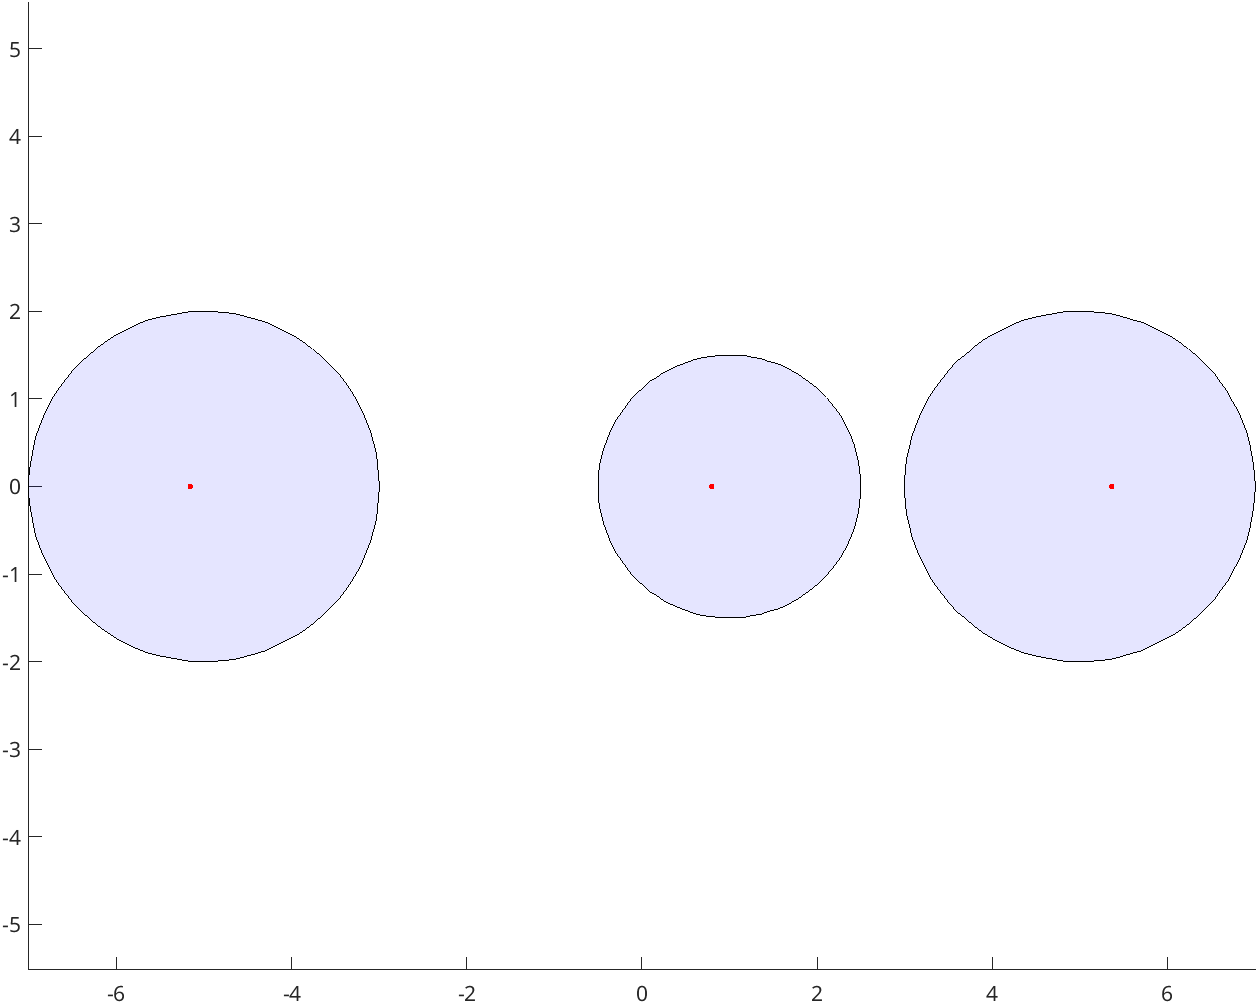
\includegraphics{../figures/gersh.png}
\end{center}

Notiamo come, nel caso specifico, a 3 cerchi di Gershgorin distinti corrispondono 3 autovalori distinti, e quindi la matrice $A$ è diagonalizzabile.
\end{document}
